%% LyX 1.6.2 created this file.  For more info, see http://www.lyx.org/.
%% Do not edit unless you really know what you are doing.
\documentclass{scrartcl}
\usepackage[usenames,dvipsnames,pdftex]{color}
\usepackage{amsmath,amssymb,amsfonts}
%\usepackage[alsoload={accepted,named,prefix}]{siunitx}
%\usepackage[load-configurations=version-1]{siunitx}
\usepackage{subeqnarray}
\usepackage[format=hang]{subfig}
\usepackage{booktabs}
\usepackage{verbatim}
\usepackage{miller}
\usepackage{bm}
\usepackage{geometry}
\usepackage[authoryear]{natbib}
%Check if we are compiling under latex or pdflatex
\ifx\pdftexversion\undefined
  \usepackage[dvips,draft]{graphicx}
\else
%  \usepackage[pdftex,draft]{graphicx}
  \usepackage[pdftex]{graphicx}
\fi
\graphicspath{
                          {./figures/}
                          {./}
                         }
\DeclareGraphicsExtensions{.pdf,.png}
\definecolor{DarkBlue}{rgb}{.106, .212, .4}

\usepackage[pdftex,%                             hyper-references for pdftex
bookmarksnumbered=true,%                         generate bookmarks with numbers
pagebackref=true,%                               generate backref in biblio
colorlinks=true,%
linkcolor=DarkBlue,citecolor=DarkBlue,urlcolor=DarkBlue%
]{hyperref}%


\begin{document}

\title{Summary of constitutive\_phenoPowerlaw}
\author{YunJo Ro \and Philip Eisenlohr}
\maketitle
\begin{abstract}
This document contains information for constitutive\_phenoPowerlaw.f90.
This constitutive subroutine is modified from the current contitutive\_phenomenological.f90.
We introduce slip and twin family as additional index (or input) for
each crystal structure in lattice.f90 subroutine (e.g., for HCP crystal:
slip and twin system has four families, respectively). 
\end{abstract}

\section{State Variables in constitutive\_phenoPowerlaw.f90}

The current State variables in constitutive\_phenoPowerlaw are {}``slip
resistance $\left(s^{\alpha}\right)$'', ''twin resistance $\left(s^{\beta}\right)$'',
{}``cumulative shear strain $\left(\gamma^{\alpha}\right)$'', and
{}``twin volume fraction $\left(f^{\beta}\right)$''. Superscript
$\alpha$ and $\beta$ denote to slip and twin systems, respectively,
in this entire document. 


\section{Considered Deformation Mechanisms}

Table \ref{Flo:DeformationSystemTable} lists slip/twin systems for
the {}``hex (hcp)'' case.\medskip{}


%
\begin{table}[tbph]
\centering
\begin{tabular}{cccc}
\toprule
 \textbf{type} & \textbf{system} & \textbf{plane / direction} & \textbf{multiplicity}\\
\midrule
slip  & basal & $\left\{ 0001\right\} \left\langle 1\bar{2}10\right\rangle $ & 3\\
 & prism & $\left\{ 10\bar{1}0\right\} \left\langle 1\bar{2}10\right\rangle $ & 3\\
 & pyr \hkl<a> & $\left\{ 10\bar{1}1\right\} \left\langle 1\bar{2}10\right\rangle $ & 6\\
 & pyr \hkl<c+a> & $\left\{ 10\bar{1}1\right\} \left\langle 2\bar{1}\bar{1}3\right\rangle $ & 12\\
\midrule
twin & T1 & $\left\{ 10\bar{1}2\right\} \left\langle \bar{1}011\right\rangle $ & 6\\
 & C1 & $\left\{ 11\bar{2}2\right\} \left\langle 11\bar{2}\bar{3}\right\rangle $ & 6\\
 & T2 & $\left\{ 11\bar{2}1\right\} \left\langle \bar{1}\bar{1}26\right\rangle $ & 6\\
 & C2 & $\left\{ 10\bar{1}1\right\} \left\langle 10\bar{1}\bar{2}\right\rangle $ & 6\\
\bottomrule
\end{tabular}\caption{Implemented deformation mechanims in $\alpha$-Ti }
\label{Flo:DeformationSystemTable}
\end{table}

Slip/twin system for HCP are illustrated in Figures \ref{fig: dislocation slip systems}
and \ref{fig: twinning systems}.


%..............FIG...............
% === SEM ===
\begin{figure}
\centering
\subfloat[Basal \hkl<a> slip]{%
\label{fig: dislocation slip basal}%
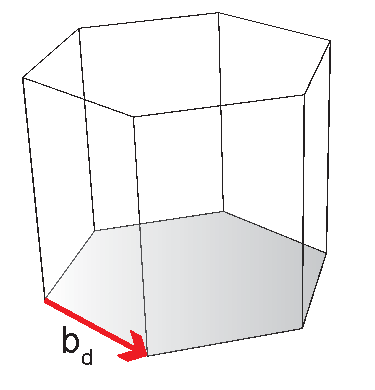
\includegraphics{slipSystem_basal}}
\quad
\subfloat[Prismatic \hkl<a> slip]{%
\label{fig: dislocation slip prism}%
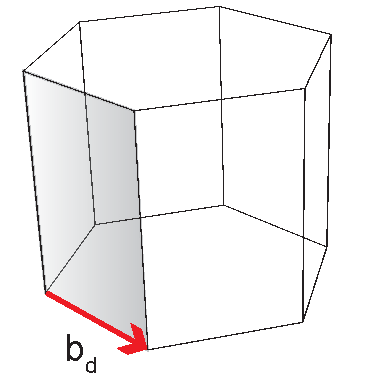
\includegraphics{slipSystem_prismA}}
\quad
\subfloat[Pyramidal \hkl<a> slip]{%
\label{fig: dislocation slip pyramidal a}%
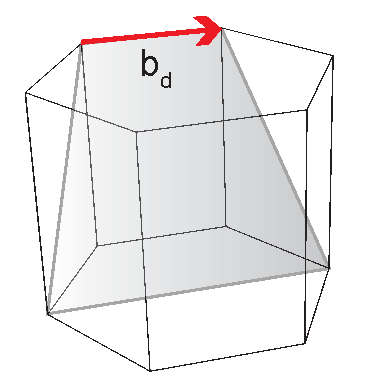
\includegraphics{slipSystem_pyrA}}
\quad
\subfloat[Pyramidal \hkl<c+a> slip]{%
\label{fig: dislocation slip pyramidal ca}%
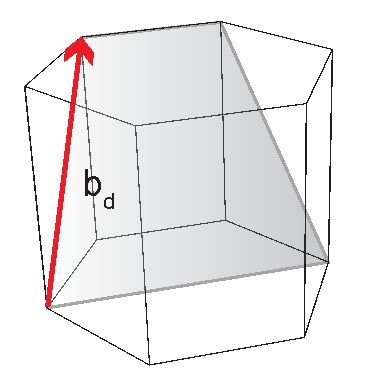
\includegraphics{slipSystem_pyrCA}}
\quad
\caption{
Dislocation slip systems considered for hexagonal lattice structure.}
\label{fig: dislocation slip systems}
\end{figure}
%...................................

%..............FIG...............
% === SEM ===
\begin{figure}
\centering
\subfloat[Extension (T1)]{%
\label{fig: twin T1}%
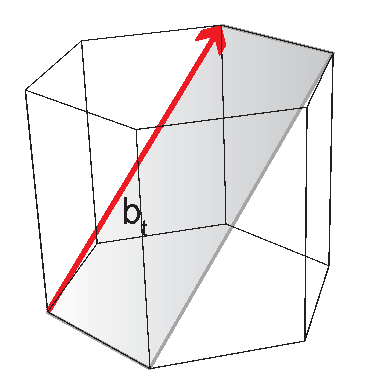
\includegraphics{twinSystem_T1}}
\quad
\subfloat[Contraction (C1)]{%
\label{fig: twin C1}%
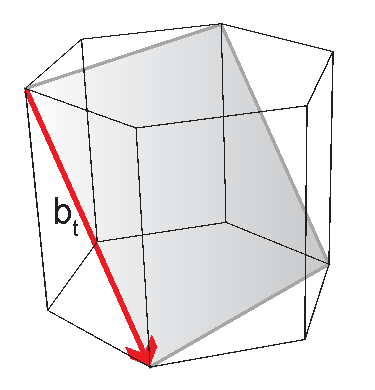
\includegraphics{twinSystem_C1}}
\quad
\subfloat[Extension (T2)]{%
\label{fig: twin T2}%
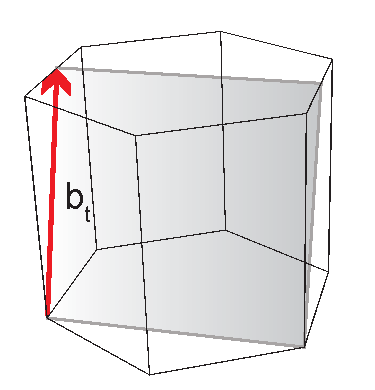
\includegraphics{twinSystem_T2}}
\quad
\subfloat[Contraction (C2)]{%
\label{fig: twin C2}%
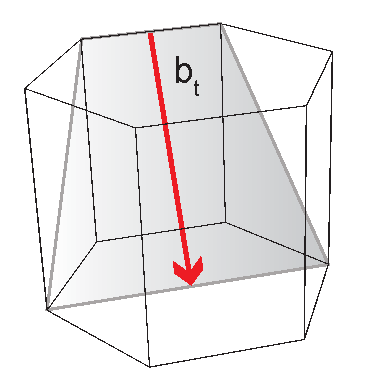
\includegraphics{twinSystem_C2}}
\quad
\caption{
Mechanical twinning systems considered for hexagonal lattice structure. Burgers vectors are not drawn to scale.}
\label{fig: twinning systems}
\end{figure}
%...................................



\section{Kinetics}

Shear strain rate due to slip is described by following equation \citet{Salem2005,Wu2007}:\begin{equation}
\dot{\gamma}^{\alpha}=\dot{\gamma_{o}}\left|\frac{\tau^{\alpha}}{s^{\alpha}}\right|^{n}sign\left(\tau^{\alpha}\right)\label{eq:slipStrainRate}\end{equation}


, where $\dot{\gamma}^{\alpha}$; shear strain rate, $\dot{\gamma}_{o}$;
reference shear strain rate, $\tau^{\alpha}$; resolved shear stress
on the slip system, $n$; stress exponent, and $s^{\alpha}$; slip
resistance.

Twin volume fraction rate is described by following equation \citet{Salem2005,Wu2007}:

\begin{equation}
\dot{f}^{\beta}=\frac{\dot{\gamma_{o}}}{\gamma^{\beta}}\left|\frac{\tau^{\beta}}{s^{\beta}}\right|^{n}\mathbb{\mathcal{H}}\left(\tau^{\beta}\right)\label{eq:twinVolrate}\end{equation}


, where $\dot{f}^{\beta}$; twin volume fraction rate, $\dot{\gamma}_{o}$;
reference shear strain rate, $\gamma^{\beta}$;shear strain due to
mechanical twinning, $\tau^{\beta}$; resolved shear stress on the
twin system, and $s^{\beta}$; twin resistance. $\mathcal{H}$ is
Heaviside function. 


\section{Structure Evolution}

In this present section, we attempt to show how we establish the relationship
between the evolutoin of slip/twin resistance and the evolution of
shear strain/twin volume fraction. 


\subsection{Interaction matrix. }

Conceptual relationship between the evolution of state and kinetic
variables is shown in Equation \ref{eq:InteractionMatrix}.

\begin{equation}
\left[\begin{array}{c}
\dot{s}^{\alpha}\\
\dot{s}^{\beta}\end{array}\right]=\left[\begin{array}{cc}
M_{\mathrm{slip-slip}} & M_{\mathrm{slip-twin}}\\
M_{\mathrm{twin-slip}} & M_{\mathrm{twin-twin}}\end{array}\right]\left[\begin{array}{c}
\dot{\gamma}^{\alpha}\\
\gamma^{\beta}\cdot\dot{f}^{\beta}\end{array}\right]\label{eq:InteractionMatrix}\end{equation}


Four interaction martices are followings; i) slip-slip interaction
matrix $\left(M_{\mathrm{{\scriptstyle slip-slip}}}\right)$, ii)
slip-twin interaction matrix $\left(M_{\mathrm{slip-twin}}\right)$,
iii) twin-slip interaction matrix $\left(M_{\mathrm{twin-slip}}\right)$,
and iv) twin-twin interaction matrix $\left(M_{\mathrm{twin-twin}}\right)$. 

Detailed interaction type matrices in Equation \ref{eq:InteractionMatrix}
will be further discussed in the following Section.


\subsection{Interaction type matrix}

Following sections are sparated into four based on each interaction
type matrix alluded. Numbers in Tables \ref{Flo:SlipSlipIntTypeTable},
\ref{Flo:SlipTwinIntTypeTable}, \ref{Flo:TwinSlipIntTypeTable},
and \ref{Flo:TwinTwinIntTypeTable} denote the type of interaction
between deformation systems (The first column vs. The first row).


\subsubsection{Slip-Slip interaction type matrix}
\begin{itemize}
\item There are 20 types of slip-slip interaction as shown in Table \ref{Flo:SlipSlipIntTypeTable}. 
\item In Table \ref{Flo:SlipSlipIntTypeTable}, types of latent hardening
among slip systems are listed. 
\item Actual slip-slip interaction type matrix, $M_{\mathrm{slip-slip}}^{'}$,
is listed in Equation \ref{eq:SlipSlipIntMatrix}.
\end{itemize}
%
\begin{table}[H]
\begin{centering}
\begin{tabular}{ccccc}
\toprule
 & basal & prism & pyr \hkl<a> & pyr\hkl<c+a>\\
\midrule
basal & 1, 5 & 9 & 12 & 14\\
prism & 15 & 2, 6 & 10 & 13\\
pyr \hkl<a> & 18 & 16 & 3, 7 & 11\\
pyr \hkl<c+a> & 20 & 19 & 17 & 4, 8\\
\bottomrule
\end{tabular}
\par\end{centering}

\caption{Slip--slip interaction type}
\label{Flo:SlipSlipIntTypeTable}
\end{table}


\begin{equation}
M_{\mathrm{slip-slip}}^{'}=\left[\begin{array}{ccc|ccc|cccccc|cccccccccccc}
1 & 5 & 5 & \cdot & \cdot & \cdot & \cdot & \cdot & \cdot & \cdot & \cdot & \cdot & \cdot & \cdot & \cdot & \cdot & \cdot & \cdot & \cdot & \cdot & \cdot & \cdot & \cdot & \cdot\\
 & 1 & 5 & \cdot & 9 & \cdot & \cdot & \cdot & 12 & \cdot & \cdot & \cdot & \cdot & \cdot & \cdot & \cdot & \cdot & 14 & \cdot & \cdot & \cdot & \cdot & \cdot & \cdot\\
 &  & 1 & \cdot & \cdot & \cdot & \cdot & \cdot & \cdot & \cdot & \cdot & \cdot & \cdot & \cdot & \cdot & \cdot & \cdot & \cdot & \cdot & \cdot & \cdot & \cdot & \cdot & \cdot\\
\hline \cdot & \cdot & \cdot & 2 & 6 & 6 & \cdot & \cdot & \cdot & \cdot & \cdot & \cdot & \cdot & \cdot & \cdot & \cdot & \cdot & \cdot & \cdot & \cdot & \cdot & \cdot & \cdot & \cdot\\
\cdot & 15 & \cdot &  & 2 & 6 & \cdot & \cdot & 10 & \cdot & \cdot & \cdot & \cdot & \cdot & \cdot & \cdot & \cdot & 13 & \cdot & \cdot & \cdot & \cdot & \cdot & \cdot\\
\cdot & \cdot & \cdot &  &  & 2 & \cdot & \cdot & \cdot & \cdot & \cdot & \cdot & \cdot & \cdot & \cdot & \cdot & \cdot & \cdot & \cdot & \cdot & \cdot & \cdot & \cdot & \cdot\\
\hline \cdot & \cdot & \cdot & \cdot & \cdot & \cdot & 3 & 7 & 7 & 7 & 7 & 7 & \cdot & \cdot & \cdot & \cdot & \cdot & \cdot & \cdot & \cdot & \cdot & \cdot & \cdot & \cdot\\
\cdot & \cdot & \cdot & \cdot & \cdot & \cdot &  & 3 & 7 & 7 & 7 & 7 & \cdot & \cdot & \cdot & \cdot & \cdot & \cdot & \cdot & \cdot & \cdot & \cdot & \cdot & \cdot\\
\cdot & \cdot & \cdot & \cdot & \cdot & \cdot &  &  & 3 & 7 & 7 & 7 & \cdot & \cdot & \cdot & \cdot & \cdot & 11 & \cdot & \cdot & \cdot & \cdot & \cdot & \cdot\\
\cdot & 18 & \cdot & \cdot & 16 & \cdot &  &  &  & 3 & 7 & 7 & \cdot & \cdot & \cdot & \cdot & \cdot & \cdot & \cdot & \cdot & \cdot & \cdot & \cdot & \cdot\\
\cdot & \cdot & \cdot & \cdot & \cdot & \cdot &  &  &  &  & 3 & 7 & \cdot & \cdot & \cdot & \cdot & \cdot & \cdot & \cdot & \cdot & \cdot & \cdot & \cdot & \cdot\\
\cdot & \cdot & \cdot & \cdot & \cdot & \cdot &  &  &  &  &  & 3 & \cdot & \cdot & \cdot & \cdot & \cdot & \cdot & \cdot & \cdot & \cdot & \cdot & \cdot & \cdot\\
\hline \cdot & \cdot & \cdot & \cdot & \cdot & \cdot & \cdot & \cdot & \cdot & \cdot & \cdot & \cdot & 4 & 8 & 8 & 8 & 8 & 8 & 8 & 8 & 8 & 8 & 8 & 8\\
\cdot & \cdot & \cdot & \cdot & \cdot & \cdot & \cdot & \cdot & \cdot & \cdot & \cdot & \cdot &  & 4 & 8 & 8 & 8 & 8 & 8 & 8 & 8 & 8 & 8 & 8\\
\cdot & \cdot & \cdot & \cdot & \cdot & \cdot & \cdot & \cdot & \cdot & \cdot & \cdot & \cdot &  &  & 4 & 8 & 8 & 8 & 8 & 8 & 8 & 8 & 8 & 8\\
\cdot & \cdot & \cdot & \cdot & \cdot & \cdot & \cdot & \cdot & \cdot & \cdot & \cdot & \cdot &  &  &  & 4 & 8 & 8 & 8 & 8 & 8 & 8 & 8 & 8\\
\cdot & 20 & \cdot & \cdot & 19 & \cdot & \cdot & \cdot & 17 & \cdot & \cdot & \cdot &  &  &  &  & 4 & 8 & 8 & 8 & 8 & 8 & 8 & 8\\
\cdot & \cdot & \cdot & \cdot & \cdot & \cdot & \cdot & \cdot & \cdot & \cdot & \cdot & \cdot &  &  &  &  &  & 4 & 8 & 8 & 8 & 8 & 8 & 8\\
\cdot & \cdot & \cdot & \cdot & \cdot & \cdot & \cdot & \cdot & \cdot & \cdot & \cdot & \cdot &  &  &  &  &  &  & 4 & 8 & 8 & 8 & 8 & 8\\
\cdot & \cdot & \cdot & \cdot & \cdot & \cdot & \cdot & \cdot & \cdot & \cdot & \cdot & \cdot &  &  &  &  &  &  &  & 4 & 8 & 8 & 8 & 8\\
\cdot & \cdot & \cdot & \cdot & \cdot & \cdot & \cdot & \cdot & \cdot & \cdot & \cdot & \cdot &  &  &  &  &  &  &  &  & 4 & 8 & 8 & 8\\
\cdot & \cdot & \cdot & \cdot & \cdot & \cdot & \cdot & \cdot & \cdot & \cdot & \cdot & \cdot &  &  &  &  &  &  &  &  &  & 4 & 8 & 8\\
\cdot & \cdot & \cdot & \cdot & \cdot & \cdot & \cdot & \cdot & \cdot & \cdot & \cdot & \cdot &  &  &  &  &  &  &  &  &  &  & 4 & 8\\
\cdot & \cdot & \cdot & \cdot & \cdot & \cdot & \cdot & \cdot & \cdot & \cdot & \cdot & \cdot &  &  &  &  &  &  &  &  &  &  &  & 4\end{array}\right]\label{eq:SlipSlipIntMatrix}\end{equation}


\vfill{}
\vfill{}



\subsubsection{Slip-Twin interaction type matrix}
\begin{itemize}
\item There are 16 types of slip-twin interaction in Table \ref{Flo:SlipTwinIntTypeTable}. 
\item Meaning of T1, C1, T2, C2 is listed in Table \ref{Flo:DeformationSystemTable}.
\item Actual slip-twin interaction type matrix, $M_{\mathrm{slip-twin}}^{'}$,
is listed in Equation \ref{eq:SlipTwinIntMatrix}.
\end{itemize}
%
\begin{table}[H]
\begin{centering}
\begin{tabular}{ccccc}
\toprule 
 & T1 & C1 & T2 & C1\\
\midrule
basal & 1 & 2 & 3 & 4\\
prism & 5 & 6 & 7 & 8\\
pyr \hkl<a> & 9 & 10 & 11 & 12\\
pyr \hkl<c+a> & 13 & 14 & 15 & 16\\
\bottomrule
\end{tabular}
\par\end{centering}

\caption{Slip-twin interaction type}
\label{Flo:SlipTwinIntTypeTable}
\end{table}


\begin{equation}
M_{\mathrm{slip-twin}}^{'}=\left[\begin{array}{c|c|c|c}
1 & 2 & 3 & 4\\
\hline 5 & 6 & 7 & 8\\
\hline 9 & 10 & 11 & 12\\
\hline 13 & 14 & 15 & 16\end{array}\right]\label{eq:SlipTwinIntMatrix}\end{equation}



\subsubsection{Twin-Slip interaction type matrix}
\begin{itemize}
\item There 16 types of twin-slip interaction in Table \ref{Flo:TwinSlipIntTypeTable}.
\item Meaning of T1, C1, T2, C2 is listed in Table \ref{Flo:DeformationSystemTable}.
\item Actual twin-slip interaction type matrix, $M_{\mathrm{twin-slip}}^{'}$,
is listed in Equation \ref{eq:TwinSlipIntMatrix}.
\end{itemize}
%
\begin{table}[H]
\begin{centering}
\begin{tabular}{ccccc}
\toprule 
 & basal & prism & pyr \hkl<a> & pyr \hkl<c+a>\\
 \midrule
T1 & 1 & 5 & 9 & 13\\
C1 & 2 & 6 & 10 & 14\\
T2 & 3 & 7 & 11 & 15\\
C2 & 4 & 8 & 12 & 16\\
\bottomrule
\end{tabular}
\par\end{centering}

\caption{Twin-slip interaction type}
\label{Flo:TwinSlipIntTypeTable}
\end{table}


\begin{equation}
M_{\mathrm{twin-slip}}^{'}=\left[\begin{array}{c|c|c|c}
1 & 5 & 9 & 13\\
\hline 2 & 6 & 10 & 14\\
\hline 3 & 7 & 11 & 15\\
\hline 4 & 8 & 12 & 16\end{array}\right]\label{eq:TwinSlipIntMatrix}\end{equation}



\subsubsection{Twin-twin interaction type matrix}
\begin{itemize}
\item There are 20 types of twin-twin interaction as shown in Table \ref{Flo:TwinTwinIntTypeTable}. 
\item In Table \ref{Flo:TwinTwinIntTypeTable}, types of latent hardening
among twin systems are listed. 
\item Actual twin-twin interaction type marix, $M_{\mathrm{twin-twin}}^{'}$,
is listed in Equation \ref{eq:TwinTwinIntMatrix}.
\end{itemize}
%
\begin{table}[H]
\begin{centering}
\begin{tabular}{ccccc}
\toprule 
 & T1 & C1 & T2 & C2\\
\midrule
T1 & 1, 5 & 9 & 12 & 14\\
C1 & 15 & 2, 6 & 10 & 13\\
T2 & 18 & 16 & 3, 7 & 11\\
C2 & 20 & 19 & 17 & 4, 8\\
\bottomrule
\end{tabular}
\par\end{centering}

\caption{Twin-twin interaction type}
\label{Flo:TwinTwinIntTypeTable}
\end{table}


\begin{equation}
M_{\mathrm{twin-twin}}^{'}=\left[\begin{array}{cccccc|cccccc|cccccc|cccccc}
1 & 5 & 5 & 5 & 5 & 5 & \cdot & \cdot & \cdot & \cdot & \cdot & \cdot & \cdot & \cdot & \cdot & \cdot & \cdot & \cdot & \cdot & \cdot & \cdot & \cdot & \cdot & \cdot\\
 & 1 & 5 & 5 & 5 & 5 & \cdot & \cdot & \cdot & \cdot & \cdot & \cdot & \cdot & \cdot & \cdot & \cdot & \cdot & \cdot & \cdot & \cdot & \cdot & \cdot & \cdot & \cdot\\
 &  & 1 & 5 & 5 & 5 & \cdot & \cdot & \cdot & \cdot & \cdot & \cdot & \cdot & \cdot & \cdot & \cdot & \cdot & \cdot & \cdot & \cdot & \cdot & \cdot & \cdot & \cdot\\
 &  &  & 1 & 5 & 5 & \cdot & \cdot & \cdot & 9 & \cdot & \cdot & \cdot & \cdot & \cdot & 12 & \cdot & \cdot & \cdot & \cdot & \cdot & 14 & \cdot & \cdot\\
 &  &  &  & 1 & 5 & \cdot & \cdot & \cdot & \cdot & \cdot & \cdot & \cdot & \cdot & \cdot & \cdot & \cdot & \cdot & \cdot & \cdot & \cdot & \cdot & \cdot & \cdot\\
 &  &  &  &  & 1 & \cdot & \cdot & \cdot & \cdot & \cdot & \cdot & \cdot & \cdot & \cdot & \cdot & \cdot & \cdot & \cdot & \cdot & \cdot & \cdot & \cdot & \cdot\\
\hline \cdot & \cdot & \cdot & \cdot & \cdot & \cdot & 2 & 6 & 6 & 6 & 6 & 6 & \cdot & \cdot & \cdot & \cdot & \cdot & \cdot & \cdot & \cdot & \cdot & \cdot & \cdot & \cdot\\
\cdot & \cdot & \cdot & \cdot & \cdot & \cdot &  & 2 & 6 & 6 & 6 & 6 & \cdot & \cdot & \cdot & \cdot & \cdot & \cdot & \cdot & \cdot & \cdot & \cdot & \cdot & \cdot\\
\cdot & \cdot & \cdot & \cdot & \cdot & \cdot &  &  & 2 & 6 & 6 & 6 & \cdot & \cdot & \cdot & \cdot & \cdot & \cdot & \cdot & \cdot & \cdot & \cdot & \cdot & \cdot\\
\cdot & \cdot & \cdot & 15 & \cdot & \cdot &  &  &  & 2 & 6 & 6 & \cdot & \cdot & \cdot & 10 & \cdot & \cdot & \cdot & \cdot & \cdot & 13 & \cdot & \cdot\\
\cdot & \cdot & \cdot & \cdot & \cdot & \cdot &  &  &  &  & 2 & 6 & \cdot & \cdot & \cdot & \cdot & \cdot & \cdot & \cdot & \cdot & \cdot & \cdot & \cdot & \cdot\\
\cdot & \cdot & \cdot & \cdot & \cdot & \cdot &  &  &  &  &  & 2 & \cdot & \cdot & \cdot & \cdot & \cdot & \cdot & \cdot & \cdot & \cdot & \cdot & \cdot & \cdot\\
\hline \cdot & \cdot & \cdot & \cdot & \cdot & \cdot & \cdot & \cdot & \cdot & \cdot & \cdot & \cdot & 3 & 7 & 7 & 7 & 7 & 7 & \cdot & \cdot & \cdot & \cdot & \cdot & \cdot\\
\cdot & \cdot & \cdot & \cdot & \cdot & \cdot & \cdot & \cdot & \cdot & \cdot & \cdot & \cdot &  & 3 & 7 & 7 & 7 & 7 & \cdot & \cdot & \cdot & \cdot & \cdot & \cdot\\
\cdot & \cdot & \cdot & \cdot & \cdot & \cdot & \cdot & \cdot & \cdot & \cdot & \cdot & \cdot &  &  & 3 & 7 & 7 & 7 & \cdot & \cdot & \cdot & \cdot & \cdot & \cdot\\
\cdot & \cdot & \cdot & 18 & \cdot & \cdot & \cdot & \cdot & \cdot & 16 & \cdot & \cdot &  &  &  & 3 & 7 & 7 & \cdot & \cdot & \cdot & 11 & \cdot & \cdot\\
\cdot & \cdot & \cdot & \cdot & \cdot & \cdot & \cdot & \cdot & \cdot & \cdot & \cdot & \cdot &  &  &  &  & 3 & 7 & \cdot & \cdot & \cdot & \cdot & \cdot & \cdot\\
\cdot & \cdot & \cdot & \cdot & \cdot & \cdot & \cdot & \cdot & \cdot & \cdot & \cdot & \cdot &  &  &  &  &  & 3 & \cdot & \cdot & \cdot & \cdot & \cdot & \cdot\\
\hline \cdot & \cdot & \cdot & \cdot & \cdot & \cdot & \cdot & \cdot & \cdot & \cdot & \cdot & \cdot & \cdot & \cdot & \cdot & \cdot & \cdot & \cdot & 4 & 8 & 8 & 8 & 8 & 8\\
\cdot & \cdot & \cdot & \cdot & \cdot & \cdot & \cdot & \cdot & \cdot & \cdot & \cdot & \cdot & \cdot & \cdot & \cdot & \cdot & \cdot & \cdot &  & 4 & 8 & 8 & 8 & 8\\
\cdot & \cdot & \cdot & \cdot & \cdot & \cdot & \cdot & \cdot & \cdot & \cdot & \cdot & \cdot & \cdot & \cdot & \cdot & \cdot & \cdot & \cdot &  &  & 4 & 8 & 8 & 8\\
\cdot & \cdot & \cdot & 20 & \cdot & \cdot & \cdot & \cdot & \cdot & 19 & \cdot & \cdot & \cdot & \cdot & \cdot & 17 & \cdot & \cdot &  &  &  & 4 & 8 & 8\\
\cdot & \cdot & \cdot & \cdot & \cdot & \cdot & \cdot & \cdot & \cdot & \cdot & \cdot & \cdot & \cdot & \cdot & \cdot & \cdot & \cdot & \cdot &  &  &  &  & 4 & 8\\
\cdot & \cdot & \cdot & \cdot & \cdot & \cdot & \cdot & \cdot & \cdot & \cdot & \cdot & \cdot & \cdot & \cdot & \cdot & \cdot & \cdot & \cdot &  &  &  &  &  & 4\end{array}\right]\label{eq:TwinTwinIntMatrix}\end{equation}



\subsection{Prefactor (nonlinear factor)}


\subsubsection{Prefactors for slip resistance $\left(s^{\alpha}\right)$; $M_{\mathrm{slip-slip}}$
and $M_{\mathrm{slip-twin}}$\citet{Wu2007}}

$M_{\mathrm{slip-slip}}$ and $M_{\mathrm{slip-twin}}$ use for slip
resistance evolution $\left(\dot{s}^{\alpha}\right)$. Equation \ref{eq:SlipResisEvolutionEq}
is for a slip resistance rate evolution. This currently shows the
prefactor for {}``slip-slip interaction matrix, $M_{\mathrm{slip-slip}}$''.

\medskip{}


\begin{equation}
M_{\mathrm{slip-slip}}=h_{\mathrm{slip}}\left(1+C\cdot F^{b}\right)\left(1-\frac{s^{\alpha}}{s_{so}^{\alpha}+s_{\mathrm{pr}}\cdot\sqrt{F}}\right)\cdot M_{\mathrm{slip-slip}}^{'}\label{eq:SlipResisEvolutionEq}\end{equation}


\medskip{}


, where $h_{\mathrm{slip}}$represent a hardening rate, and $S_{\mathrm{so}}^{\alpha}$
saturation slip resistance for slip system without mechanical twinning
$\left(\sum_{\beta}f^{\beta}=0\right)$, respectively. And, $F$ is
$\sum_{\beta}f^{\beta}$, and $N^{S}$is the total number of slip
system.$C$, $s_{\mathrm{pr}}$, and $b$ are coefficients to introduce
the effect of interaction between slip and mechanical twin in Equation
\ref{eq:SlipResisEvolutionEq}.
\begin{itemize}
\item Slip-twin interaction matrix, $M_{\mathrm{slip-twin}}$, has not been
implemented with any prefactor in the present version. 
\end{itemize}

\subsubsection{Prefactors for twin resistance $\left(s^{\beta}\right)$; $M_{\mathrm{twin-slip}}$
and $M_{\mathrm{twin-twin}}$\citet{Salem2005}}

$M_{\mathrm{twin-sli}p}$ and $M_{\mathrm{twin-twin}}$ use for twin
resistance evolution $\left(\dot{s}^{\beta}\right)$. Twin-twin and
twin-slip interaction matrices are described in Equations \ref{eq:TwinTwinContributionToTwinResis}
and \ref{eq:TwinSlipContributionToTwinResis}. \medskip{}


\begin{equation}
M_{\mathrm{twin-twin}}=h_{\mathrm{tw}}\cdot F^{d}\cdot M_{\mathrm{twin-twin}}^{'}\label{eq:TwinTwinContributionToTwinResis}\end{equation}


,where $h_{\mathrm{tw}}$ and $d$ are coefficients for twin-twin
contribution. $F$ is $\sum_{\beta}f^{\beta}$.

\medskip{}


\begin{equation}
M_{\mathrm{twin-slip}}=h_{\mathrm{tw-sl}}\cdot\Gamma^{e}\cdot M_{\mathrm{twin-slip}}^{'}\label{eq:TwinSlipContributionToTwinResis}\end{equation}


,where $h_{\mathrm{tw-sl}}$ and $e$ are coefficients for twin-slip
contribution, and $\Gamma=\sum_{\alpha}\gamma^{\alpha}$.

\clearpage{}


\section{Material Parameters (Material Configuration file)}

%
\begin{figure}[tbph]
\begin{centering}
\includegraphics[clip,scale=0.6]{figures/ExpectedMaterialConfigFile}\caption{Expected of phenomenological modelling parameters.}
\label{Fig:ModelParameters}
\par\end{centering}


\end{figure}

\begin{itemize}
\item The sequence for hardening coefficients in Figure \ref{Fig:ModelParameters}
is the sequence of numbering in Tables \ref{Flo:SlipSlipIntTypeTable},
\ref{Flo:SlipTwinIntTypeTable}, \ref{Flo:TwinSlipIntTypeTable},
and \ref{Flo:TwinTwinIntTypeTable} above.
\end{itemize}

\clearpage{}
\bibliographystyle{plainnat}
\bibliography{MPIEyjr}

\end{document}
